\documentclass[a4paper,12pt]{article}
%\documentclass[fleqn]{article}

% ---パッケージ---
\usepackage{amsmath,amssymb}    %数式用
\usepackage{tcolorbox}   %囲み枠用(tcolorboxに変更)
\usepackage{geometry}   %余白調節
\usepackage{tikz}  % ← 図を描くためのTikZパッケージ
\geometry{margin=25mm}  %余白を少し狭く
\usetikzlibrary{decorations.pathmorphing,patterns,positioning,arrows.meta} % バネ・壁の模様
\tikzset{
  block/.style = {draw, rectangle, minimum height=2em, minimum width=3em},
  sum/.style = {draw, circle, inner sep=0pt, minimum size=5mm},
  input/.style = {coordinate},
  output/.style = {coordinate}
}
\usetikzlibrary{calc}

% --- 日本語用パッケージ ---
\usepackage{luatexja}         % 日本語表示に必要
\usepackage{luatexja-fontspec} % フォント指定用

% --- フォント指定(Overleaf標準フォント)---
\setmainjfont{IPAexMincho}  % 明朝体
%\setmainjfont{IPAexGothic}  % ゴシック体にしたい場合

% --- tcolorbox の設定 ---
\tcbset{
  colframe=black,
  colback=white,         % 本文の背景(白)
  boxrule=0.8pt,
  arc=3pt,
  outer arc=3pt,
  boxsep=4pt,
  coltitle=black,
  colbacktitle=gray!20,  % タイトルの背景(グレー)
  fonttitle=\normalsize
}

\begin{document}

\begin{titlepage}
    \centering
    \vspace*{2cm}
    {\LARGE {制御工学演習} \par}
    \vspace{1cm}
    {\Large 問題編 \par}
    \vfill
    \begin{flushright}
      \large
      作成者:Yudai\\
      2025年5月9日作成
    \end{flushright}
\end{titlepage}

\noindent
[1] 指数関数 \(x(t) =e^{at}\) をラプラス変換せよ.\\
\vspace{10mm}


\noindent
[2] 単位ステップ関数 \( x(t) = 1 \) をラプラス変換せよ.\\
\vspace{10mm}


\noindent
[3] 単位インパルス関数 \( x(t) = \delta(t) \)をラプラス変換せよ.\\
\vspace{10mm}


\noindent
[4] ランプ関数 \( x(t) = t \) をラプラス変換せよ.\\
\vspace{10mm}


\noindent
[5] 正弦波関数 \( x(t) = \sin(\omega t) \) をラプラス変換せよ.\\
\vspace{10mm}


\noindent
[6] 余弦波関数 \( x(t) = \cos(\omega t) \) をラプラス変換せよ.\\
\vspace{10mm}


\noindent
[7] ラプラス変換は線形の性質があることを示せ. \\
\vspace{10mm}


\noindent
[8] 時間関数\( x(t) \)を右に \tau だけ推移させた関数\( x(t - \tau) \)に対するラプラス変換は,\\
\quad \( x(t) \) のラプラス変換 \( X(s)\) を用いて 
\vspace{-2mm}
\begin{align*}
    \mathcal{L} \left[ x(t - \tau) \right] &=
    e^{-s
    \tau t}X(s)
\end{align*}
\quad と表されることを示せ.(時間領域における推移定理)\\
\vspace{10mm}


\noindent
[9]  \( x(t) \) のラプラス変換\( X(s) \)において複素変数\(s\)を\(b\)だけ推移させて \(s+b\) \\
\quad とすれば,どうなるのか? \\
\vspace{10mm}


\noindent
[10] \( e^{\lambda t} sin(\omega t) \) をラプラス変換せよ.\\
\vspace{10mm}

\newpage

\noindent
[11] 時間関数 \( x(t) \) の微分をラプラス変換せよ.\\
\vspace{10mm}


\noindent
[12] つぎの微分方程式をラプラス変換を用いて解け.
\[
    9 \frac{d^2 x(t)}{dt^2} + x(t) = 1 
\]
\quad ただし,初期値は,$x(0) = 0,\ x'(0) = 0$ とする.\\
\vspace{10mm}


\noindent
[13] つぎの微分方程式をラプラス変換を用いて解け.\\
\[
\frac{d^2 x(t)}{dt^2} + 3 \frac{dx(t)}{dt} + 2x(t) = 4
\]
\quad ただし,初期条件は,$x(0)=1,\ x^{(1)}(0)=0$ とする.\\
\vspace{10mm}


\noindent
[14] つぎの微分方程式をラプラス変換を用いて解け.\\
\[
\frac{dx(t)}{dt} + 3x(t) = sin{2t}
\]
\quad ただし,初期条件は,$x(0)=0$ とする.\\
\vspace{10mm}


\noindent
[15] つぎの微分方程式をラプラス変換を用いて解け.\\
\[
\frac{d^2 x(t)}{dt^2} + 2\frac{dx(t)}{dt} + 2x(t) = 1 \\
\]
\quad ただし,初期条件は,$x(0)=0 , x^{1}(0)=1$ とする.\\
\vspace{10mm}

\newpage


\noindent
[16] (1)-(10)のラプラス変換$X(s)$にラプラス逆変換を施し,時間関数$x(t)$を求めよ.\\
\[
\renewcommand{\arraystretch}{3.0} % ← 行の高さ倍率を変更(1.0が標準)
\begin{tabular}{@{}rl@{\quad\quad}rl@{}}
(1) & $X(s)=\frac{4}{s+5}$                          &(2) & $X(s)=\frac{ s + 7 }{ s^2 + 2s + 5}$ \\
(3) & $X(s)=\frac{ 2 }{ s^2 + s }$                  &(4) & $X(s)=\frac{ s + 1 }{ s ( s^2 + 4s + 8 )}$ \\
(5) & $X(s)=\frac{ 1 }{ s^3 + 11 s^2+ 40s + 48 }$   &(6) & $X(s)=\frac{ 2 }{ ( s + 1 ) ( s + 3 ) }$ \\
(7) & $X(s)=\frac{ 3 }{ s ( s + 2)^2 }$             &(8) & $X(s)=\frac{ 1 }{ s ( s + 2 ) ( s + 3 )^2 }$ \\
(9) & $X(s)=\frac{ s + 2 }{s^3 ( s - 1 )^2 }$       &(10)& $X(s)=\frac{ 1 }{ ( s^2 + 1 ) ( s^2 + 4 ) }$ \\
\end{tabular}
\]
\vspace{10mm}


\noindent
[17] つぎの微分方程式をラプラス変換を用いて解け.\\
\[
\frac{d^2y(t)}{dt^2} + y(t) = 0
\]
\quad ただし,初期条件は,\(y(0)=A, y^{(1)}(0)=B\) とする.
\vspace{10mm}


\noindent
[18] つぎの微分方程式をラプラス変換を用いて解け.\\
\[
\frac{d^2y(t)}{dt^2} -( a + b )\frac{dy(t)}{dt} + a b y(t) = 0
\]
\quad ただし,初期条件は,\(y(0)=1, y^{(1)}(0)=0\) とする.
\vspace{10mm}


\noindent
[19] つぎの微分方程式をラプラス変換を用いて解け.\\
\[
\frac{d^2y(t)}{dt^2} - \frac{dy(t)}{dt} - 12 y(t) = 2
\]
\quad ただし,初期条件は,\(y(0)=1, y^{(1)}(0)=0\) とする.
\vspace{10mm}


\noindent
[20] つぎの微分方程式をラプラス変換を用いて解け.\\
\[
\frac{d^2y(t)}{dt^2} + 4 y(t) = sin(t)
\]
\quad ただし,初期条件は,\(y(0)=0, y^{(1)}(0)=0\) とする.
\vspace{10mm}


\noindent
[21] 単位インパルス応答が\(y(t)=7e^{-2t}+2e^{-3t}\)であるとき,\\ 
\qquad このシステムの伝達関数を求めよ.
\vspace{10mm}


\noindent
[22] 単位インパルス応答が\(y(t)=e^{-2t}+3e^{-9t}-4e^{-11t}\)であるとき,\\
\qquad このシステムの伝達関数を求めよ.
\vspace{10mm}


\noindent
[23] 単位ステップ応答が\(y(t)=5e^{-t}-5e^{-7t}\)であるとき,\\
\qquad このシステムの伝達関数を求めよ.
\vspace{10mm}


\noindent
[24] 単位ステップ応答が\(y(t)=12+6t\)であるとき,\\
\qquad このシステムの伝達関数を求めよ.
\vspace{10mm}


\noindent
[25] 伝達関数が
\[G(s)=\frac{2}{s^2+3s+2}\]
\qquad であるときのインパルス応答を求めよ.
\vspace{10mm}


\noindent
[26] 伝達関数が
\[G(s)=\frac{2}{s^2+3s+2}\]
\qquad であるときのステップ応答を求めよ.
\vspace{10mm}


\noindent
[27] 伝達関数が
\[G(s)=\frac{12s+30}{s^2+8s+15}\]
\qquad であるときのステップ応答を求めよ.
\vspace{10mm}


\noindent
[28] \(x(t)[m^3/s]\)は,操作バルブ直後の流量を表し,
長い配管を通って\\
\qquad \(L[s]\)後に給水場所に到達したとする.\\
\qquad このとき,\(x(t)\)から給水量\(y(t)\)までの伝達関数を求めよ.
\vspace{10mm}


\newpage


\noindent
[29] 変位\(x_i(t)[m]\)を入力信号,\\
\qquad ダッシュポットのシリンダの平衡点からの変位\(x_o(t)[m]\)を出力信号\\
\qquad とみなしたときの伝達関数を求めよ.ただし,\(x_i(0)= 0, x_o(0)=0\)とする.
\begin{center}
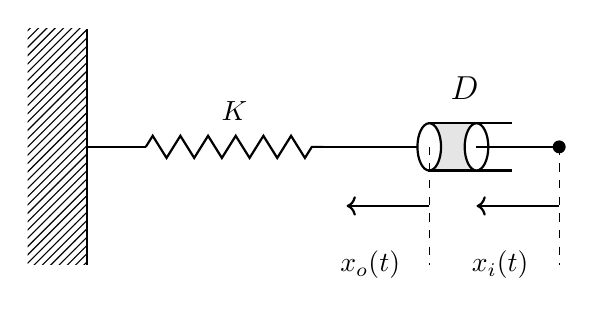
\begin{tikzpicture}[scale=1.5]
% 固定壁
\fill[pattern=north east lines] (-0.5,0) rectangle (0,2);
\draw[thick] (0,0) -- (0,2);

% バネ
\draw[thick] (0,1) -- (0.5,1);
\draw[thick, decorate, decoration={zigzag, segment length=10, amplitude=4}] (0.5,1) -- (2,1);
\node at (1.25,1.3) {$K$};

% --- ダンパー(シリンダー形) ---
\draw[thick] (2,1) -- (2.9,1); % 棒(変更なし)
\draw[thick, fill=gray!20] (2.9,0.8) rectangle (3.3,1.2); % 筒の側面
\draw[thick] (3.3,1.2) -- (3.6,1.2);% 筒の側面(上)
\draw[thick] (3.3,0.8) -- (3.6,0.8);% 筒の側面(下)
\draw[thick, fill=white] (2.9,1) ellipse (0.1 and 0.2);   % 左側の端面(楕円)
\draw[thick, fill=white] (3.3,1) ellipse (0.1 and 0.2);   % 右側の端面(楕円)
\draw[thick] (3.3,1) -- (4.0,1); % ピストン棒 → 始点を 3.5 → 3.3 に変更
\node at (3.2,1.5) {\large $D$};


% 入力矢印
\draw[->, thick] (4,0.5) -- (3.3,0.5);
\node at (3.5,0) {$x_i(t)$};

% 出力矢印
\draw[->, thick] (2.9,0.5) -- (2.2,0.5);
\node at (2.4,0) {$x_o(t)$};

% 支点
\draw[fill] (4,1) circle (0.05);

% 点線
\draw[dashed] (2.9,1) -- (2.9,0);
\draw[dashed] (4.0,1) -- (4.0,0);
\end{tikzpicture}
\end{center}


\noindent
[30] 外力\(f(t)[N]\)を図の方向に考え,平衡点からの変位\(x(t)[m]\)を出力信号\\
\qquad とみなしたときの伝達関数を求めよ. 
\begin{center}
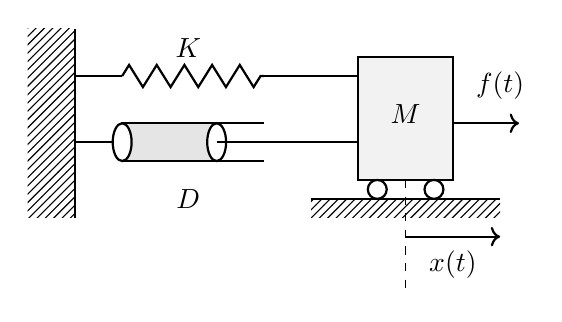
\begin{tikzpicture}[scale=1.2]
% 固定壁
\fill[pattern=north east lines] (-0.5,0) rectangle (0,2);
\draw[thick] (0,0) -- (0,2);

% バネ
\draw[thick] (0,1.5) -- (0.5,1.5);
\draw[thick, decorate, decoration={zigzag, segment length=10, amplitude=4}] (0.5,1.5) -- (2,1.5);
\draw[thick] (2,1.5) -- (3.5,1.5);
\node at (1.2,1.8) {$K$};

% ダンパー(シリンダー形式)
\draw[thick] (0,0.8) -- (0.5,0.8); % 棒
\draw[thick, fill=gray!20] (0.5,0.6) rectangle (1.5,1.0); % 筒の側面
\draw[thick] (1.5,1.0) -- (2,1.0); % 筒の上
\draw[thick] (1.5,0.6) -- (2,0.6); % 筒の下
\draw[thick, fill=white] (0.5,0.8) ellipse (0.1 and 0.2); % 左端面
\draw[thick, fill=white] (1.5,0.8) ellipse (0.1 and 0.2); % 右端面
\draw[thick] (1.5,0.8) -- (3,0.8); % ピストン棒
\node at (1.2,0.2) {$D$};

% 質量M
\draw[thick, fill=gray!10] (3,0.4) rectangle (4,1.7);
\node at (3.5,1.1) {$M$};
% ローラー追加
    \draw[thick] (3.2,0.3) circle (0.1);
    \draw[thick] (3.8,0.3) circle (0.1);


% 床
\draw[thick] (2.5,0.2) -- (4.5,0.2);
\fill[pattern=north east lines] (2.5,0) rectangle (4.5,0.2);

% 座標
\draw[->, thick] (3.5,-0.2) -- (4.5,-0.2);
\node at (4,-0.5) {$x(t)$};
\draw[dashed] (3.5,0.4) -- (3.5,-0.8);

% 外力
\draw[->, thick] (4,1) -- (4.7,1);
\node at (4.5,1.4) {$f(t)$};
\end{tikzpicture}
\end{center}


\noindent
[31] 平衡点からの変位として,図中の\(x_i(t)[m]\)と\(x_o(t)[m]\)を考える.\\
\qquad \(x_i(t)\)を入力信号,\(x_o(t)[m]\) を出力信号とみなしたときの伝達関数を求めよ.
\begin{center}
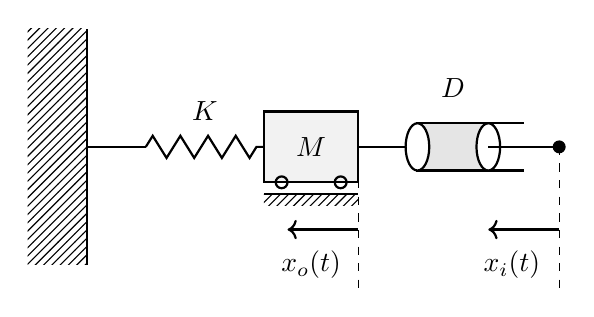
\begin{tikzpicture}[scale=1.5]
    % 固定壁
    \fill[pattern=north east lines] (-0.5,0) rectangle (0,2);
    \draw[thick] (0,0) -- (0,2);

    % バネ
    \draw[thick] (0,1) -- (0.5,1);
    \draw[thick, decorate, decoration={zigzag, segment length=10, amplitude=4}] (0.5,1) -- (1.5,1);
    \node at (1,1.3) {$K$};

    % 質量M
    \draw[thick, fill=gray!10] (1.5,0.7) rectangle (2.3,1.3);
    \node at (1.9,1) {$M$};
    % ローラー
    \draw[thick] (1.65,0.7) circle (0.05);
    \draw[thick] (2.15,0.7) circle (0.05);
    % 地面
    \draw[thick] (1.5,0.6) -- (2.3,0.6);
    \fill[pattern=north east lines] (1.5,0.5) rectangle (2.3,0.6);

    % ダンパー
    \draw[thick] (2.3,1) -- (2.8,1); % 棒
    \draw[thick, fill=gray!20] (2.8,0.8) rectangle (3.4,1.2); % 筒
    \draw[thick] (3.4,1.2) -- (3.7,1.2); % 筒上
    \draw[thick] (3.4,0.8) -- (3.7,0.8); % 筒下
    \draw[thick, fill=white] (2.8,1) ellipse (0.1 and 0.2);
    \draw[thick, fill=white] (3.4,1) ellipse (0.1 and 0.2);
    \draw[thick] (3.4,1) -- (4,1); % ピストン棒
    \node at (3.1,1.5) {$D$};

    % 入力矢印
    \draw[->, thick] (4,0.3) -- (3.4,0.3);
    \node at (3.6,0) {$x_i(t)$};

    % 出力矢印
    \draw[->, thick] (2.3,0.3) -- (1.7,0.3);
    \node at (1.9,0) {$x_o(t)$};

    % 支点
    \draw[fill] (4,1) circle (0.05);

    % 点線
    \draw[dashed] (2.3,1) -- (2.3,-0.2);
\draw[dashed] (4,1) -- (4,-0.2);
\end{tikzpicture}
\end{center}


\noindent
[32] 粘性減衰係数\(D_1[N \cdot s /m]\)のダッシュポットのピストンの平衡点からの変位\\
\qquad \(x_i(t)[m]\)を入力信号,粘性減衰係数\(D_1[N \cdot s /m]\)のダッシュポットのピストン \\
\qquad の平衡点からの   変位\(x_o(t)[m]\) を出力信号としたときの伝達関数を求めよ.
\begin{center}
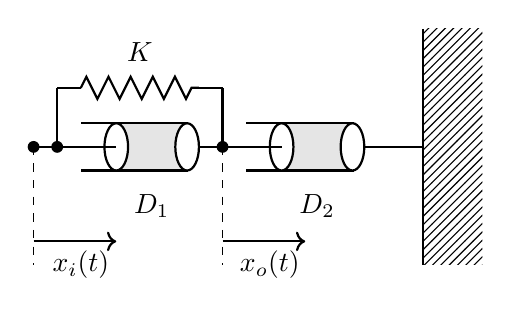
\begin{tikzpicture}[scale=1.5]
% 固定壁
\fill[pattern=north east lines] (4,0) rectangle (4.5,2);
\draw[thick] (4,2) -- (4,0);

% ダンパ D2
\draw[thick, fill=gray!20] (2.8,0.8) rectangle (3.4,1.2);
\draw[thick] (2.8,1.2) -- (2.5,1.2);
\draw[thick] (2.8,0.8) -- (2.5,0.8);
\draw[thick, fill=white] (2.8,1) ellipse (0.1 and 0.2);
\draw[thick, fill=white] (3.4,1) ellipse (0.1 and 0.2);
\draw[thick] (2,1) -- (2.8,1);
\draw[thick] (3.5,1) -- (4,1);
\node at (3.1,0.5) {$D_2$};

% ダンパ D1
\draw[thick, fill=gray!20] (1.4,0.8) rectangle (2.0,1.2);
\draw[thick] (1.4,1.2) -- (1.1,1.2);
\draw[thick] (1.4,0.8) -- (1.1,0.8);
\draw[thick, fill=white] (1.4,1) ellipse (0.1 and 0.2);
\draw[thick, fill=white] (2.0,1) ellipse (0.1 and 0.2);
\draw[thick] (0.7,1) -- (1.4,1);
\node at (1.7,0.5) {$D_1$};

% バネ K
\draw[thick] (0.9,1) -- (0.9,1.5);
\draw[thick] (0.9,1.5) -- (1.1,1.5);
\draw[thick, decorate, decoration={zigzag, segment length=8, amplitude=4}] (1.1,1.5) -- (2.1,1.5);
\draw[thick] (2.1,1.5) -- (2.3,1.5);
\draw[thick] (2.3,1) -- (2.3,1.5);
\node at (1.6,1.8) {$K$};

% 接点
\fill (0.7,1) circle (0.05);
\fill (0.9,1) circle (0.05);
\fill (2.3,1) circle (0.05);


% 点線(基準線)
\draw[dashed] (0.7,1) -- (0.7,0);
\draw[dashed] (2.3,1) -- (2.3,0);

% 入力 x₁(t)
\draw[->, thick] (0.7,0.2) -- (1.4,0.2);
\node at (1.1,0) {$x_{i}(t)$};

% 出力 x₂(t)
\draw[->, thick] (2.3,0.2) -- (3,0.2);
\node at (2.7,0) {$x_{o}(t)$};
\end{tikzpicture}
\end{center}


\newpage


\noindent
[33] 平衡点からの変位として,図中の\(x_i(t)[m]\)と\(x_o(t)[m]\)を考える. \\
\qquad \(x_i(t)[m]\)を入力信号,\(x_o(t)[m]\)を出力信号とみなしたときの伝達巻子を求めよ.\\
\qquad 台車は摩擦なく床を動くものとする.すべての変数の初期値はゼロである.
\begin{center}
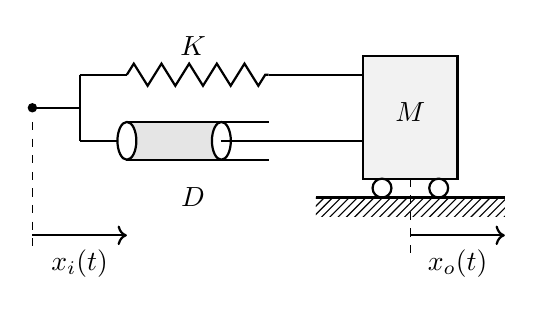
\begin{tikzpicture}[scale=1.2]
    % バネ
    \draw[thick] (0,1.5) -- (0.5,1.5);
    \draw[thick, decorate, decoration={zigzag, segment length=10, amplitude=4}] (0.5,1.5) -- (2,1.5);
    \draw[thick] (2,1.5) -- (3.5,1.5);
    \node at (1.2,1.8) {$K$};

    % ダンパー(シリンダー形式)
    \draw[thick] (0,0.8) -- (0.5,0.8); % 棒
    \draw[thick, fill=gray!20] (0.5,0.6) rectangle (1.5,1.0); % 筒の側面
    \draw[thick] (1.5,1.0) -- (2,1.0); % 筒の上
    \draw[thick] (1.5,0.6) -- (2,0.6); % 筒の下
    \draw[thick, fill=white] (0.5,0.8) ellipse (0.1 and 0.2); % 左端面
    \draw[thick, fill=white] (1.5,0.8) ellipse (0.1 and 0.2); % 右端面
    \draw[thick] (1.5,0.8) -- (3,0.8); % ピストン棒
    \node at (1.2,0.2) {$D$};

    % 質量M
    \draw[thick, fill=gray!10] (3,0.4) rectangle (4,1.7);
    \node at (3.5,1.1) {$M$};
    % ローラー追加
    \draw[thick] (3.2,0.3) circle (0.1);
    \draw[thick] (3.8,0.3) circle (0.1);

    % 床
    \draw[thick] (2.5,0.2) -- (4.5,0.2);
    \fill[pattern=north east lines] (2.5,0) rectangle (4.5,0.2);

    % 座標
    \draw[->, thick] (3.5,-0.2) -- (4.5,-0.2);
    \node at (4,-0.5) {$x_o(t)$};
    \draw[dashed] (3.5,0.4) -- (3.5,-0.4);

    \draw[->, thick] (-0.5,-0.2) -- (0.5,-0.2);
    \node at (0,-0.5) {$x_i(t)$};
    \draw[dashed] (-0.5,1) -- (-0.5,-0.4);

    \draw[thick] (0,0.8) -- (0,1.5);
    \draw[thick] (0,1.15) -- (-0.5,1.15);

    \fill (-0.5,1.15) circle (0.05);

\end{tikzpicture}
\end{center}


\noindent
[34]この系の伝達関数を求めよ.ただし,fは粘性抵抗係数であり,\\
\qquad 初期条件\(t = 0\)において\(F=0\)
\begin{center}
    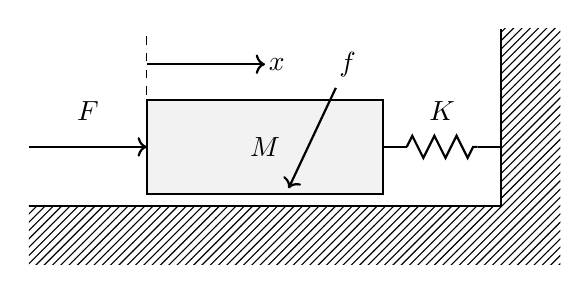
\begin{tikzpicture}[scale=1.5]
        % 固定壁
        \draw[thick] (4,2) -- (4,0.5);
        \fill[pattern=north east lines] (4,0) rectangle (4.5,2);
    
        % バネ
        \draw[thick] (3,1) -- (3.2,1);
        \draw[thick, decorate, decoration={zigzag, segment length=8, amplitude=4}] (3.2,1) -- (3.8,1);
        \draw[thick] (3.8,1) -- (4,1);
        \node at (3.5,1.3) {$K$};
    
        % 質量M
        \draw[thick, fill=gray!10] (1,0.6) rectangle (3,1.4);
        \node at (2,1) {$M$};

        %粘性抵抗係数
        \draw[->, thick] (2.6,1.5) -- (2.2,0.65);
        \node at (2.7,1.7) {$f$};

        % 地面
        \draw[thick] (0,0.5) -- (4,0.5);
        \fill[pattern=north east lines] (0,0) rectangle (4,0.5);
    
        % 外力
        \draw[->, thick] (0,1) -- (1,1);
        \node at (0.5,1.3) {$F$};
    
        % 点線
        \draw[dashed] (1,0.6) -- (1,2);
    
        % 座標
        \draw[->, thick] (1,1.7) -- (2,1.7);
        \node at (2.1,1.7) {$x$};
    \end{tikzpicture}
\end{center}


\noindent
[35] 長さ\(y_0\)のばねの上端を固定し,下端に質量\(M\)の物体をつり下げたとき,\\
\qquad ばねの長さが\(y_1\)になって平衡した.\\
\qquad つぎに,物体に下向きの力\(F(t)\) を加えたとき,物体の平衡状態からの変位を\\
\qquad \(y\)として運動方程式を作れ.\\
\qquad ただし物体と側壁との間には,粘性摩擦定数を\(f\)とする.

\begin{center}
\begin{tikzpicture}[scale=1.2]
% 左側(平衡状態)
\node at (-2,-1)[scale=0.6] {$質量-ばね-まさつ系(平衡状態)$};

    %壁
    \draw[thick] (-3,0) -- (-3,4);
    \draw[thick] (-3,4) -- (-1,4);
    \draw[thick] (-1,0) -- (-1,4);
    \fill[pattern=north east lines] (-3.5,0) rectangle (-3,4);
    \fill[pattern=north east lines] (-3.5,4) rectangle (-0.5,4.5);
    \fill[pattern=north east lines] (-1,0) rectangle (-0.5,4);


    %ばね
    \draw[thick] (-2,1) -- (-2,2);
    \draw[thick, decorate, decoration={coil, segment length=6}] (-2,2) -- (-2,3);
    \draw[thick] (-2,3) -- (-2,4);
    \node at (-2.3,2.5) {$K$};

    %重り
    \draw[thick, fill=gray!10] (-2.9,0.2) rectangle (-1.1,1);
    \node at (-2,0.6) {$M$};

    %粘性摩擦定数
    \draw[->, thick] (-1.3,0) -- (-1.1,0.6);
    \node at (-1.4,-0.2) {$f$};

    %重り
    \draw[dashed] (-2.9,1.2) rectangle (-1.1,2);

    %座標
    \draw[dashed] (-4.5,4) -- (-3,4);
    \draw[dashed] (-4.5,1) -- (-2.9,1);
    \draw[dashed] (-4,2) -- (-2.9,2);

    \draw[<->,thick] (-3.8,4) -- (-3.8,2);
    \node at (-3.95,3) {$y_0$};
    \draw[<->,thick] (-4.3,4) -- (-4.3,1);
    \node at (-4.45,2.5) {$y_1$};
    
    % 左側(平衡状態)
    \node at (2,-1)[scale=0.6] {$力を加えた場合$};

    %壁
    \draw[thick] (3,0) -- (3,4);
    \draw[thick] (3,4) -- (1,4);
    \draw[thick] (1,0) -- (1,4);
    \fill[pattern=north east lines] (3.5,0) rectangle (3,4);
    \fill[pattern=north east lines] (3.5,4) rectangle (0.5,4.5);
    \fill[pattern=north east lines] (1,0) rectangle (0.5,4);


    %ばね
    \draw[thick] (2,1.3) -- (2,2.2);
    \draw[thick, decorate, decoration={coil, segment length=6}] (2,2.2) -- (2,3.1);
    \draw[thick] (2,3.1) -- (2,4);
    \node at (2.3,2.65) {$K$};

    %重り
    \draw[thick, fill=gray!10] (2.9,0.5) rectangle (1.1,1.3);
    \node at (2,0.9) {$M$};

    %粘性摩擦定数
    \draw[->, thick] (2.7,0) -- (2.9,0.6);
    \node at (2.6,-0.2) {$f$};

    %座標
    \draw[dashed] (0.1,4) -- (1,4);
    \draw[dashed] (0.1,1.3) -- (1.1,1.3);
    \draw[dashed] (2.9,1.3) -- (4,1.3);

    \draw[<->,thick] (0.3,4) -- (0.3,1.3);
    \node at (0,2.65) {$y_1$};

    \draw[->,thick] (3.8,1.3) -- (3.8,0.5);
    \node at (3.8,0.3) {$y$};

    

\end{tikzpicture}
\end{center}


\noindent
[36] 質量\(M\)の物体の一端にばねをつけ,\\
\qquad ばねを力\(F\)で引っ張ったときの運動方程式を作れ.  \\
\qquad 物体と床面との間の粘性摩擦定数を\(f\)とする.

\begin{center}
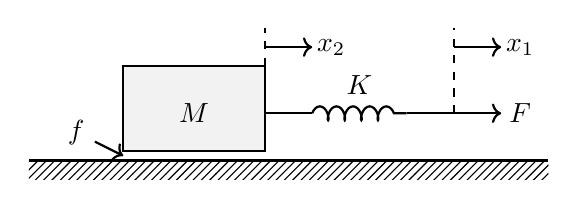
\begin{tikzpicture}[scale=1.2]
% 地面
\draw[thick] (-0.5,0) -- (5,0);
\fill[pattern=north east lines] (-0.5,-0.2) rectangle (5,0);

% 質量M
\draw[thick, fill=gray!10] (0.5,0.1) rectangle (2,1);
\node at (1.25,0.5) {$M$};
\draw[dashed] (2,1.0) -- (2,1.4);

% 摩擦f
\draw[->,thick] (0.2,0.2) -- (0.5,0.05);
\node at (0,0.3) {$f$};

% バネ
\draw[thick] (2,0.5) -- (2.5,0.5);
\draw[thick, decorate, decoration={coil, segment length=6}] (2.5,0.5) -- (3.5,0.5);
\node at (3,0.8) {$K$};
\draw[dashed] (4,0.5) -- (4,1.4);

% 外力
\draw[->, thick] (3.5,0.5) -- (4.5,0.5);
\node at (4.7,0.5) {$F$};

% 座標 x2
\draw[->, thick] (2,1.2) -- (2.5,1.2);
\node at (2.7,1.2) {$x_2$};

% 座標 x1
\draw[->, thick] (4,1.2) -- (4.5,1.2);
\node at (4.7,1.2) {$x_1$};
\end{tikzpicture}
\end{center}


\noindent
[37] 等価変換によってひとつのブロックに簡単化せよ.
\begin{center}

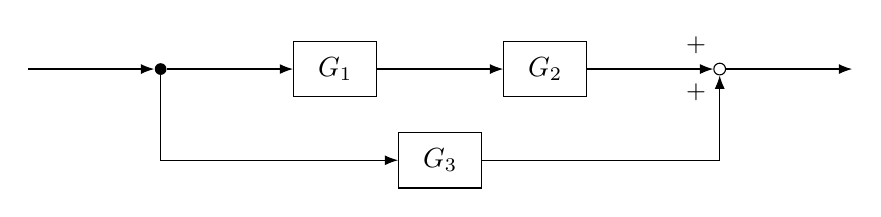
\begin{tikzpicture}[auto, node distance=1.2cm and 1.6cm, >=Latex]

% --- ノード定義 ---
\node[input] (input) {};
\node[circle, fill=black, inner sep=1.5pt, right=of input] (branch) {};     % 分岐点
\node[block, right=of branch] (G1) {$G_1$};
\node[block, right=of G1] (G2) {$G_2$};
\node[circle, draw, inner sep=1.5pt, right=of G2] (sum) {};                % 合流点
\node[output, right=of sum] (output) {};

\node[block, below=0.8cm of $(G1)!0.5!(G2)$] (G3) {$G_3$};                 % G3(下)

% --- 線描画 ---
\draw[->] (input) -- (branch);
\draw[->] (branch) -- (G1);
\draw[->] (G1) -- (G2);
\draw[->] (G2) -- (sum);
\draw[->] (sum) -- (output);

\draw[->] (branch) |- (G3);
\draw[->] (G3) -| (sum);

% --- 加算記号 ---
\node at ($(sum)+(-0.3,0.3)$) {\small $+$};
\node at ($(sum)+(-0.3,-0.3)$) {\small $+$};

\end{tikzpicture}


\end{center}


\noindent
[38] 等価変換によってひとつのブロックに簡単化せよ. 
\begin{center}
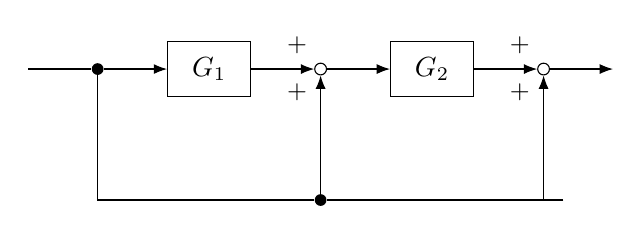
\begin{tikzpicture}[auto, node distance=1.2cm and 0.8cm, >=Latex]

% ノード定義
\node[input] (input) {};
\node[circle, fill=black, inner sep=1.5pt, minimum size=3pt, right=of input] (branch) {}; % 分岐点:黒丸(サイズ修正)

\node[block, right=of branch] (G1) {$G_1$};
\node[circle, draw, inner sep=1.5pt, minimum size=3pt, right=of G1] (sum1) {}; % 中間合流点:白丸

\node[block, right=of sum1] (G2) {$G_2$};
\node[circle, draw, inner sep=1.5pt, minimum size=3pt, right=of G2] (sum2) {}; % 出力直前合流点:白丸

\node[output, right=of sum2] (output) {};

\node[circle, fill=black, inner sep=1.5pt, minimum size=3pt, below=1.5cm of sum1] (branch2) {}; % 下の黒丸(サイズ修正)


% 線描画
\draw[-] (input) -- (branch);
\draw[->] (branch) -- (G1);
\draw[->] (G1) -- (sum1);
\draw[->] (sum1) -- (G2);
\draw[->] (G2) -- (sum2);
\draw[->] (sum2) -- (output);

\draw[-] (branch) |- (branch2);
\draw[->] (branch2.north) -| (sum1);

\draw[-] (branch2.east) -- ++(3.0,0); % .east を使うと右側から出る
\draw[->] ($(branch2.east)+(3.0,0)$) - | (sum2);

% 加算記号を合流点にそれぞれ配置
\node at ($(sum1)+(-0.3,0.3)$) {\small $+$};
\node at ($(sum1)+(-0.3,-0.3)$) {\small $+$};

\node at ($(sum2)+(-0.3,0.3)$) {\small $+$};
\node at ($(sum2)+(-0.3,-0.3)$) {\small $+$};

\end{tikzpicture}
\end{center}
\vspace{2mm}


\noindent
[39] 等価変換によってひとつのブロックに簡単化せよ. 
\begin{center}
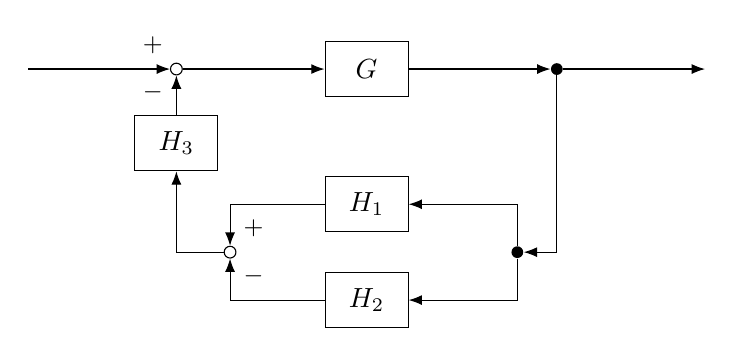
\begin{tikzpicture}[auto, node distance=1.0cm and 1.8cm, >=Latex]

% --- 上段ノード ---
\node[input] (input) {};
\node[circle, draw, inner sep=1.5pt, right=of input] (sum1) {};              % 合流点①
\node[block, right=of sum1] (G) {$G$};                                       % G
\node[circle, fill=black, inner sep=1.5pt, right=of G] (branch1) {};         % 分岐点①
\node[output, right=of branch1] (output) {};                                 % 出力

% --- H₁・H₂ 縦並び(Gの真下) ---
\node[block, below=1.0cm of G] (H1) {$H_1$};
\node[block, below=0.5cm of H1] (H2) {$H_2$};
\coordinate (midH) at ($(H1)!0.5!(H2)$);

% --- 分岐点②(右):H₁とH₂の中間、高さmidH、X位置はGとbranch1の中間よりやや右
\path (G) -- (branch1) coordinate[pos=0.6] (betweenGB);
\node[circle, fill=black, inner sep=1.5pt] at ($(midH)+(betweenGB)-(G)+(0.3,0)$) (branch2) {}; % 分岐点②

% --- 合流点②(左):midH高さ、X位置はHₛとGの中間
\node[block, below=0.5cm of sum1] (Hs) {$H_3$};                              % H_s
\path (sum1) -- (G) coordinate[pos=0.5] (leftX);
\node[circle, draw, inner sep=1.5pt] at ($(midH)+(leftX)-(G)+(-0.3,0)$) (sum2) {};  % 合流点②

% === 経路 ===
\draw[->] (input) -- (sum1);
\draw[->] (sum1) -- (G);
\draw[->] (G) -- (branch1);
\draw[->] (branch1) -- (output);

\draw[->] (branch1) |- (branch2);                 % 分岐1 → 分岐2
\draw[->] (branch2) |- (H1);                      % 分岐2 → H1(上方向)
\draw[->] (branch2) |- (H2);                      % 分岐2 → H2(下方向)

\draw[->] (H1) -| (sum2);                         % H1 → 合流2
\draw[->] (H2) -| (sum2);                         % H2 → 合流2

\draw[->] (sum2) -| (Hs);                         % 合流2 → Hs
\draw[->] (Hs) -- (sum1);                         % Hs → 合流1(フィードバック)

% --- 加算記号(揃え済) ---
\node at ($(sum1)+(-0.3,0.3)$) {\small $+$};
\node at ($(sum1)+(-0.3,-0.3)$) {\small $-$};
\node at ($(sum2)+(0.3,0.3)$) {\small $+$};
\node at ($(sum2)+(0.3,-0.3)$) {\small $-$};

\end{tikzpicture}
\end{center}


\noindent
[40] 等価変換によってひとつのブロックに簡単化せよ.
\begin{center}
\begin{tikzpicture}[auto, node distance=0.8cm and 0.8cm, >=Latex]

% --- 上段ノード(左→右) ---
\node[block] (G2) {$G_2$};
\node[circle, fill=black, inner sep=1.5pt, right=of G2] (branch1) {};     % 分岐点①
\node[circle, draw, inner sep=1.5pt, right=of branch1] (sum1) {};         % 合流点①
\node[block, right=of sum1] (G1) {$G_1$};                                 % G_1
\node[circle, fill=black, inner sep=1.5pt, right=of G1] (branch2) {};     % 分岐点②
\node[output, right=of branch2] (output) {};                              % 出力

% --- 下段ノード ---
\node[circle, draw, inner sep=1.5pt, below=1.5cm of branch1] (sum2) {};   % 合流点②
\node[input, above=1.8cm of sum1] (input) {};                             % 入力(合流点①の上)

% === 経路 ===
\draw[->] (input) -- (sum1);                       % input ↓ 合流点1
\draw[->] (sum1) -- (G1);                          % 合流点1 → G1
\draw[->] (G1) -- (branch2);                       % G1 → 分岐点2
\draw[->] (branch2) -- (output);                   % 分岐点2 → 出力

\draw[->] (branch2) |- (sum2);                     % 分岐点2 → 合流点2(下)

\draw[->] (sum2) -| ($(G2.west)+(-0.8,0)$) -- (G2); % ←↑→経路:合流点2 → 左 → 上 → G2

\draw[->] (G2) -- (branch1);                       % G2 → 分岐点1
\draw[->] (branch1) -- (sum1);                     % 分岐点1 → 合流点1
\draw[->] (branch1) -- (sum2);                     % 分岐点1 → 合流点2(短絡)

% --- 加算記号配置 ---
\node at ($(sum1)+(-0.3,0.3)$) {\small $+$};
\node at ($(sum1)+(-0.3,-0.3)$) {\small $+$};
\node at ($(sum2)+(0.3,0.3)$) {\small $+$};
\node at ($(sum2)+(0.3,-0.3)$) {\small $+$};

\end{tikzpicture}
\end{center}


\noindent
[41] 出力信号である制御量\(Y\)までの伝達特性を等価変換によって簡単化せよ.\\
\qquad ただし、\(R\)は目標値信号,\(D\)は外乱信号である.
\begin{center}
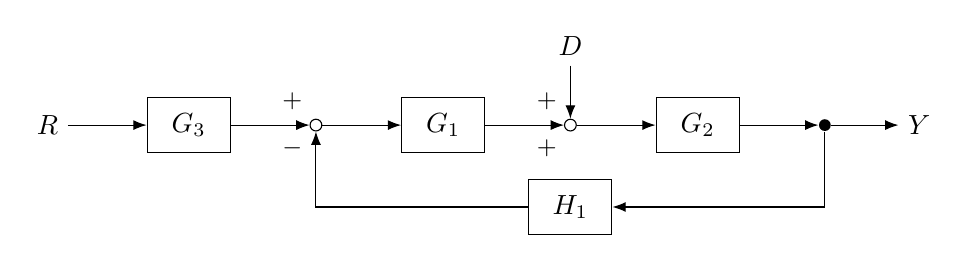
\begin{tikzpicture}[auto, node distance=0.8cm and 1.0cm, >=Latex]

% --- ノードと信号配置(横並び) ---
\node at (0,0) (R) {$R$};                           % R(目標値)
\node[block, right=of R] (G3) {$G_3$};              % G3
\node[circle, draw, inner sep=1.5pt, right=of G3] (sum1) {};  % 合流点1
\node[block, right=of sum1] (G1) {$G_1$};           % G1
\node[circle, draw, inner sep=1.5pt, right=of G1] (sum2) {};  % 合流点2
\node[block, right=of sum2] (G2) {$G_2$};           % G2
\node[circle, fill=black, inner sep=1.5pt, right=of G2] (branch) {}; % 分岐点
\node at ($(branch)+(1.2,0)$) (Y) {$Y$};             % Y(制御量)

% --- 上下ノード ---
\node at ($(sum2)+(0,1.0)$) (D) {$D$};               % D(外乱)
\node[block, below=0.6cm of sum2] (H1) {$H_1$};      % H1(下)

% === 経路 ===
\draw[->] (R) -- (G3);
\draw[->] (G3) -- (sum1);
\draw[->] (sum1) -- (G1);
\draw[->] (G1) -- (sum2);
\draw[->] (sum2) -- (G2);
\draw[->] (G2) -- (branch);
\draw[->] (branch) -- (Y);

\draw[->] (D) -- (sum2);            % D → 合流点2
\draw[->] (branch) |- (H1);         % 分岐 → H1(下)
\draw[->] (H1) -| (sum1);           % H1 → 合流点1(戻る)

% --- 加算記号配置 ---
\node at ($(sum1)+(-0.3,0.3)$) {\small $+$};
\node at ($(sum1)+(-0.3,-0.3)$) {\small $-$};
\node at ($(sum2)+(-0.3,0.3)$) {\small $+$};
\node at ($(sum2)+(-0.3,-0.3)$) {\small $+$};

\end{tikzpicture}
\end{center}


\newpage


\noindent
[42] \(a\)を入力,\(b\)を出力としたとき,ブロック線図を簡単化し,伝達関数を求めよ. 
\begin{center}
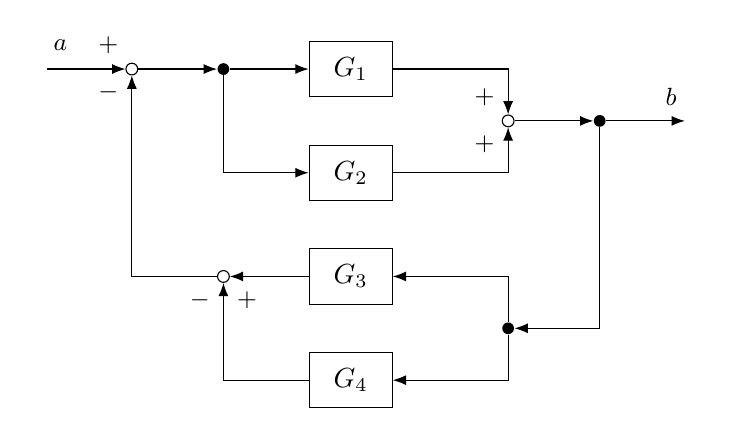
\begin{tikzpicture}[auto, node distance=0.8cm and 1.0cm, >=Latex]

% --- 上段:主系列ノード ---
\node at (0,0) (input) {};
\node[circle, draw, inner sep=1.5pt, right=of input] (sum1) {};               % 合流1
\node[circle, fill=black, inner sep=1.5pt, right=of sum1] (branch1) {};       % 分岐1
\node[block, right=of branch1] (G1) {$G_1$};                                   % G1

% --- 縦系列:G2〜G4 ---
\node[block, below=0.6cm of G1] (G2) {$G_2$};
\node[block, below=0.6cm of G2] (G3) {$G_3$};
\node[block, below=0.6cm of G3] (G4) {$G_4$};

% --- G1とG2の中間に sum2 → branch2 → output ---
\coordinate (mid12) at ($(G1)!0.5!(G2)$);
\node[circle, draw, inner sep=1.5pt] at ($(mid12)+(2.0,0)$) (sum2) {};        % 合流2
\node[circle, fill=black, inner sep=1.5pt, right=of sum2] (branch2) {};       % 分岐2
\node[right=of branch2] (output) {};

% --- G3とG4の中間に branch3 ---
\coordinate (mid34) at ($(G3)!0.5!(G4)$);
\node[circle, fill=black, inner sep=1.5pt] at ($(mid34)+(2.0,0)$) (branch3) {}; % 分岐3

% --- branch1の下かつG3の左に合流3 ---
\node[circle, draw, inner sep=1.5pt, left=of G3] (sum3) {};% 合流3

% === 経路 ===
\draw[->] (input) -- (sum1);
\draw[->] (sum1) -- (branch1);
\draw[->] (branch1) -- (G1);
\draw[->] (G1) -| (sum2);
\draw[->] (sum2) -- (branch2);
\draw[->] (branch2) -- (output);

\draw[->] (branch1) |- (G2);
\draw[->] (G2) -| (sum2);

\draw[->] (branch2) |- (branch3);
\draw[->] (branch3) |- (G3);
\draw[->] (G3) -- (sum3);
\draw[->] (sum3) -| (sum1);

\draw[->] (branch3) |- (G4);
\draw[->] (G4) -| (sum3);

% --- 加算記号 ---
\node at ($(sum1)+(-0.3,0.3)$) {\small $+$};
\node at ($(sum1)+(-0.3,-0.3)$) {\small $-$};
\node at ($(sum2)+(-0.3,0.3)$) {\small $+$};
\node at ($(sum2)+(-0.3,-0.3)$) {\small $+$};
\node at ($(sum3)+(-0.3,-0.3)$) {\small $-$};
\node at ($(sum3)+(0.3,-0.3)$) {\small $+$};

% --- その他記号 ---
\node at ($(input)+(0.3,0.3)$) {\small $a$};
\node at ($(output)+(-0.3,0.3)$) {\small $b$};

\end{tikzpicture}
\end{center}


\noindent
[43] 伝達関数\(\frac{b(s)}{a(s)}\)を求めよ. 
\begin{center}
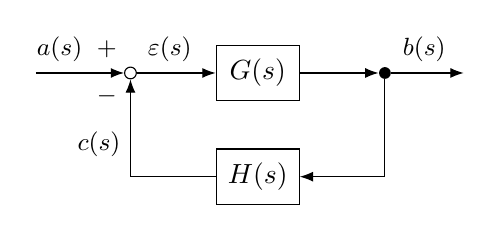
\begin{tikzpicture}[auto, node distance=0.8cm and 1.0cm, >=Latex]

% --- 横並びノード ---
\node[circle, draw, inner sep=1.5pt] (sum) {};                  % 合流点
\node[block, right=of sum] (G) {$G(s)$};                        % G(s)
\node[circle, fill=black, inner sep=1.5pt, right=of G] (branch) {};  % 分岐点

% --- 下段ノード ---
\node[block, below=0.6cm of G] (H) {$H(s)$};                    % H(s)

% --- 経路 ---
\draw[->] ++(-1.2,0) -- (sum);              % input → 合流点
\draw[->] (sum) -- (G);                     % 合流点 → G(s)
\draw[->] (G) -- (branch);                  % G(s) → 分岐点
\draw[->] (branch) -- ++(1.0,0);            % 分岐点 → output

\draw[->] (branch) |- (H);                  % 分岐点 → H(s)
\draw[->] (H) -| (sum);                     % H(s) → 合流点

% --- 加算記号 ---
\node at ($(sum)+(-0.3,0.3)$) {\small $+$};
\node at ($(sum)+(-0.3,-0.3)$) {\small $-$};

% --- その他記号 ---
\node at ($(sum)+(-0.9,0.3)$) {\small $a(s)$};
\node at ($(sum)+(0.5,0.3)$) {\small $\varepsilon(s)$};
\node at ($(branch)+(0.5,0.3)$) {\small $b(s)$};
\node at ($(sum)+(-0.4,-0.9)$) {\small $c(s)$};
\end{tikzpicture}
\end{center}


\noindent
[44] 二つの入力信号\(a_1(s),a_2(s)\)をもつ,制御系の応答\(b(s)\)を求めよ.
\begin{center}
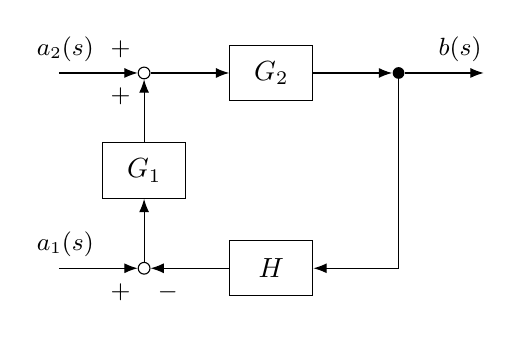
\begin{tikzpicture}[auto, node distance=0.8cm and 1.0cm, >=Latex]

    % --- 上段ノード(横並び) ---
    \node[circle, draw, inner sep=1.5pt] (sum1) {};                % 合流点1
    \node[block, right=of sum1] (G1) {$G_2$};                      % G1
    \node[circle, fill=black, inner sep=1.5pt, right=of G1] (branch) {}; % 分岐点

    % input1とoutputの位置(描かない)
    \coordinate[left=of sum1] (input1);
    \coordinate[right=of branch] (output);

    % --- 中央の縦ノード(合流1 → G2 → 合流2) ---
    \node[block, below=0.8cm of sum1] (G2) {$G_1$};                % G2
    \node[circle, draw, inner sep=1.5pt, below=0.8cm of G2] (sum2) {}; % 合流点2

    % --- 下段(横並び) ---
    \coordinate[left=of sum2] (input2);                            % input2(描かない)
    \node[block, right=of sum2] (H) {$H$};                         % H

    % === 経路 ===
    \draw[->] (input1) -- (sum1);          % input1 → 合流点1
    \draw[->] (sum1) -- (G1);              % 合流点1 → G1
    \draw[->] (G1) -- (branch);            % G1 → 分岐点
    \draw[->] (branch) -- (output);        % 分岐点 → 出力

    \draw[->] (branch) |- (H);             % 分岐点 → H
    \draw[->] (H) -- (sum2);               % H → 合流点2
    \draw[->] (sum2) -- (G2);              % 合流点2 → G2
    \draw[->] (G2) -- (sum1);              % G2 → 合流点1

    \draw[->] (input2) -- (sum2);          % input2 → 合流点2

    % --- 加算記号配置 ---
    \node at ($(sum1)+(-0.3,0.3)$) {\small $+$};
    \node at ($(sum1)+(-0.3,-0.3)$) {\small $+$};
    \node at ($(sum2)+(-0.3,-0.3)$) {\small $+$};
    \node at ($(sum2)+(0.3,-0.3)$) {\small $-$};

    % --- その他記号配置 ---
    \node at ($(sum1)+(-1.0,0.3)$) {\small $a_2(s)$};
    \node at ($(sum2)+(-1.0,0.3)$) {\small $a_1(s)$};
    \node at ($(output)+(-0.3,0.3)$) {\small $b(s)$};

\end{tikzpicture}
\end{center}


\noindent
[45] \(\frac{b_1(s)}{a_1(s)}\),\(\frac{b_1(s)}{a_2(s)}\),\(\frac{b_2(s)}{a_1(s)}\),\(\frac{b_2(s)}{a_2(s)}\)を求めよ. 
\vspace{-4mm}
\begin{center}
    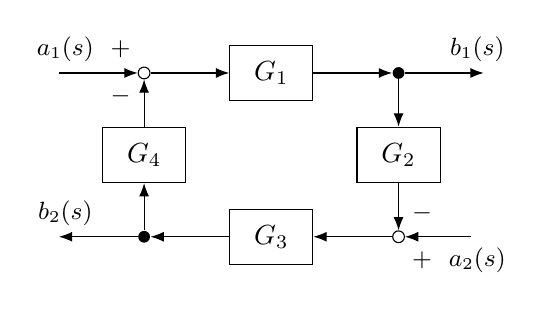
\begin{tikzpicture}[auto, node distance=0.8cm and 1.0cm, >=Latex]

% === 上段主系列(横) ===
\coordinate (input1);
\node[circle, draw, inner sep=1.5pt, right=of input1] (sum1) {};           % 合流点1
\node[block, right=of sum1] (G1) {$G_1$};                                  % G1
\node[circle, fill=black, inner sep=1.5pt, right=of G1] (branch1) {};      % 分岐点1
\coordinate[right=of branch1] (output1);                                   % 出力1(描画しない)

% === sum1の下:G4 → branch2(縦) ===
\node[block, below=0.6cm of sum1] (G4) {$G_4$};
\node[circle, fill=black, inner sep=1.5pt, below=0.6cm of G4] (branch2) {}; % 分岐点2

% === branch1の下:G2 → sum2(縦) ===
\node[block, below=0.6cm of branch1] (G2) {$G_2$};
\node[circle, draw, inner sep=1.5pt, below=0.6cm of G2] (sum2) {};          % 合流点2

% === 下段横系列:output2 ← branch2 ← G3 ← sum2 ← input2 ===
\coordinate[left=of branch2] (output2);
\node[block, right=of branch2] (G3) {$G_3$};
\coordinate[right=of G3] (sum2_right);
\coordinate[right=of sum2_right] (input2);

% === 経路 ===
\draw[->] (input1) -- (sum1);             % input1 → sum1
\draw[->] (sum1) -- (G1);                 % sum1 → G1
\draw[->] (G1) -- (branch1);              % G1 → branch1
\draw[->] (branch1) -- (output1);         % branch1 → output1

\draw[->] (input2) -- (sum2);       % input2 → sum2(右から)
\draw[->] (sum2_right) -- (G3);           % → G3
\draw[->] (G3) -- (branch2);              % G3 → branch2
\draw[->] (branch2) -- (output2);         % branch2 → output2

\draw[->] (branch1) -- (G2);              % 分岐1 → G2
\draw[->] (G2) -- (sum2);                 % G2 → 合流2

\draw[->] (branch2) -- (G4);              % 分岐2 → G4
\draw[->] (G4) -- (sum1);                 % G4 → 合流1

% === 加算記号 ===
\node at ($(sum1)+(-0.3,0.3)$) {\small $+$};
\node at ($(sum1)+(-0.3,-0.3)$) {\small $-$};
\node at ($(sum2)+(0.3,0.3)$) {\small $-$};
\node at ($(sum2)+(0.3,-0.3)$) {\small $+$};

% === その他記号 ===
\node at ($(sum1)+(-1.0,0.3)$) {\small $a_1(s)$};
\node at ($(branch1)+(1.0,0.3)$) {\small $b_1(s)$};
\node at ($(sum2)+(1.0,-0.3)$) {\small $a_2(s)$};
\node at ($(branch2)+(-1.0,0.3)$) {\small $b_2(s)$};

    \end{tikzpicture}
\end{center}


\noindent
[46] ブロック線図を簡単にせよ.
\vspace{-12mm}
\begin{center}
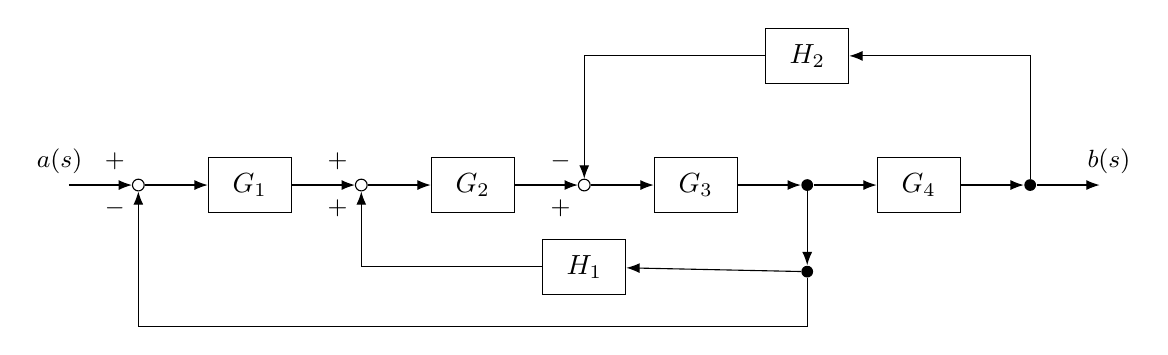
\begin{tikzpicture}[auto, node distance=0.6cm and 0.8cm, >=Latex]

% --- 主系列ノード(横並び) ---
\coordinate (input);
\node[circle, draw, inner sep=1.5pt, right=of input] (sum1) {};        % 合流1
\node[block, right=of sum1] (G1) {$G_1$};                               % G1
\node[circle, draw, inner sep=1.5pt, right=of G1] (sum2) {};           % 合流2
\node[block, right=of sum2] (G2) {$G_2$};                               % G2
\node[circle, draw, inner sep=1.5pt, right=of G2] (sum3) {};           % 合流3
\node[block, right=of sum3] (G3) {$G_3$};                               % G3
\node[circle, fill=black, inner sep=1.5pt, right=of G3] (branch1) {};  % 分岐1
\node[block, right=of branch1] (G4) {$G_4$};                            % G4
\node[circle, fill=black, inner sep=1.5pt, right=of G4] (branch2) {};  % 分岐2
\coordinate[right=of branch2] (output);

% --- 上下ノード配置 ---
\node[block, above=1.2cm of branch1] (H2) {$H_2$};                      % H2(分岐1の上)
\node[block, below=of sum3] (H1) {$H_1$};                         % H1(合流3の下)
\node[circle, fill=black, inner sep=1.5pt] at ($(branch1)+(0,-1.1)$) (branch3) {};% 分岐3(分岐1の下)

% --- 経路①: input → ... → output ---
\draw[->] (input) -- (sum1);
\draw[->] (sum1) -- (G1);
\draw[->] (G1) -- (sum2);
\draw[->] (sum2) -- (G2);
\draw[->] (G2) -- (sum3);
\draw[->] (sum3) -- (G3);
\draw[->] (G3) -- (branch1);
\draw[->] (branch1) -- (G4);
\draw[->] (G4) -- (branch2);
\draw[->] (branch2) -- (output);

% --- 経路②: 分岐2 → H2 → 合流3 ---
\draw[->] (branch2) |- (H2);
\draw[->] (H2) -| (sum3);

% --- 経路③: 分岐1 → 分岐3 → H1 → 合流2 ---
\draw[->] (branch1) -- (branch3);
\draw[->] (branch3) -- (H1);
\draw[->] (H1) -| (sum2);

% --- 経路④: 分岐3 → ↓←↑ → 合流1 ---
\coordinate (pivot) at ($(sum1)+(0,-1.8)$); % 合流点1の下
\draw[->] (branch3) |-(pivot) -- (sum1);

% --- 加算記号配置 ---
\node at ($(sum1)+(-0.3,0.3)$) {\small $+$};
\node at ($(sum1)+(-0.3,-0.3)$) {\small $-$};
\node at ($(sum2)+(-0.3,0.3)$) {\small $+$};
\node at ($(sum2)+(-0.3,-0.3)$) {\small $+$};
\node at ($(sum3)+(-0.3,0.3)$) {\small $-$};
\node at ($(sum3)+(-0.3,-0.3)$) {\small $+$};

% --- その他記号配置 ---
\node at ($(sum1)+(-1.0,0.3)$) {\small $a(s)$};
\node at ($(branch2)+(1.0,0.3)$) {\small $b(s)$};

\end{tikzpicture}
\end{center}
\vspace{2mm}


\newpage


\noindent
[47] ブロック線図を簡単にせよ. 
\begin{center}
    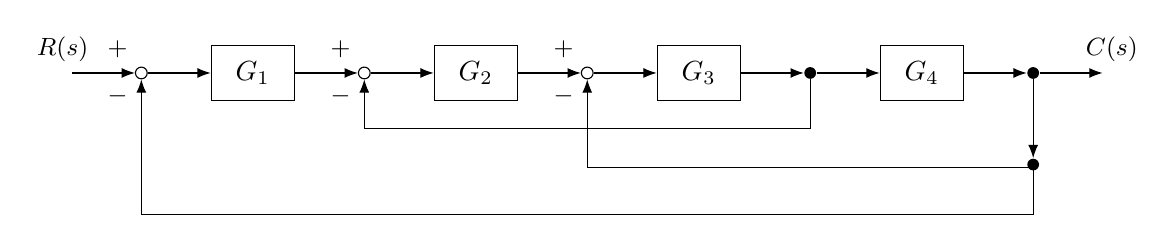
\begin{tikzpicture}[auto, node distance=0.8cm and 0.8cm, >=Latex]
    % --- 横並びの主系列ノード ---
    \node at (0,0) (input) {};
    \node[circle, draw, inner sep=1.5pt, right=of input] (sum1) {};           % 合流点1
    \node[block, right=of sum1] (G1) {$G_1$};
    \node[circle, draw, inner sep=1.5pt, right=of G1] (sum2) {};             % 合流点2
    \node[block, right=of sum2] (G2) {$G_2$};
    \node[circle, draw, inner sep=1.5pt, right=of G2] (sum3) {};             % 合流点3
    \node[block, right=of sum3] (G3) {$G_3$};
    \node[circle, fill=black, inner sep=1.5pt, right=of G3] (branch1) {};    % 分岐点1
    \node[block, right=of branch1] (G4) {$G_4$};
    \node[circle, fill=black, inner sep=1.5pt, right=of G4] (branch2) {};    % 分岐点2
    \node[right=of branch2] (output) {};
    
    % --- 分岐点3(branch2の下) ---
    \node[circle, fill=black, inner sep=1.5pt, below=1.0cm of branch2] (branch3) {};
    
    % === 主系列経路 ===
    \draw[->] (input) -- (sum1);
    \draw[->] (sum1) -- (G1);
    \draw[->] (G1) -- (sum2);
    \draw[->] (sum2) -- (G2);
    \draw[->] (G2) -- (sum3);
    \draw[->] (sum3) -- (G3);
    \draw[->] (G3) -- (branch1);
    \draw[->] (branch1) -- (G4);
    \draw[->] (G4) -- (branch2);
    \draw[->] (branch2) -- (output);
    
    % === 追加経路 ===
        % 分岐1 → 合流2(カクカク経路:下→左→上)
        \coordinate (pivot12) at ($(sum2)+(0,-0.7)$); 
        \draw[->] (branch1) |- (pivot12) -| (sum2);
    
        % 分岐2 → 分岐3(真下に新ノード) ←既に実装済
        \draw[->] (branch2) -- (branch3);
    
        % 分岐3 → 合流3(カクカク経路:下→左→上)
        \coordinate (pivot33) at ($(sum3)+(0,-1.2)$);
        \draw[->] (branch3) |- (pivot33) -| (sum3);              
    
    % 分岐3 → 合流1(カクカク:下→左→上、1本の矢印で)
    \coordinate (pivot) at ($(sum1)+(0,-1.8)$);
    \draw[->] (branch3) |- (pivot) -| (sum1);
    
    
    % --- 加算記号配置 ---
    \node at ($(sum1)+(-0.3,0.3)$) {\small $+$};
    \node at ($(sum1)+(-0.3,-0.3)$) {\small $-$};
    \node at ($(sum2)+(-0.3,0.3)$) {\small $+$};
    \node at ($(sum2)+(-0.3,-0.3)$) {\small $-$};
    \node at ($(sum3)+(-0.3,0.3)$) {\small $+$};
    \node at ($(sum3)+(-0.3,-0.3)$) {\small $-$};
    
    \node at ($(sum1)+(-1.0,0.3)$) {\small $R(s)$};
    \node at ($(branch2)+(1.0,0.3)$) {\small $C(s)$};
    
\end{tikzpicture}
\end{center}
\vspace{2mm}


\noindent
[48] ブロック線図を簡単にせよ. 
\begin{center}
    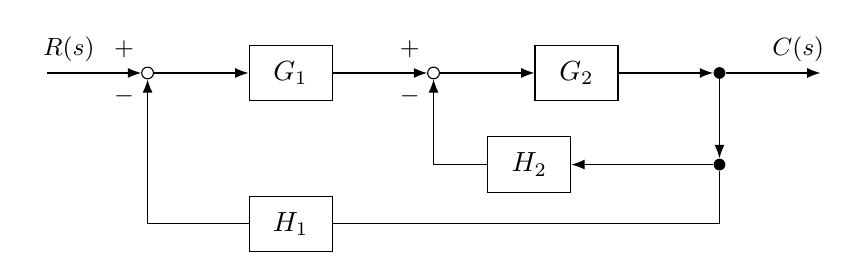
\begin{tikzpicture}[auto, node distance=0.8cm and 1.2cm, >=Latex]

    % --- 横並びの主系列ノード ---
    \node at (0,0) (input) {};
    \node[circle, draw, inner sep=1.5pt, right=of input] (sum1) {};           % 合流点1
    \node[block, right=of sum1] (G1) {$G_1$};
    \node[circle, draw, inner sep=1.5pt, right=of G1] (sum2) {};             % 合流点2
    \node[block, right=of sum2] (G2) {$G_2$};
    \node[circle, fill=black, inner sep=1.5pt, right=of G2] (branch1) {};    % 分岐点1
    \node[right=of branch1] (output) {};                                     % 出力

    % --- 下部ノード配置 ---
    \node[circle, fill=black, inner sep=1.5pt, below=1.0cm of branch1] (branch2) {}; % 分岐点2
    \node[block, left=1.8cm of branch2] (H2) {$H_2$};                                 % H2
    \node[block, below=1.2cm of G1] (H1) {$H_1$};                                     % H1(H2より下)

    % === 主系列経路 ===
    \draw[->] (input) -- (sum1);
    \draw[->] (sum1) -- (G1);
    \draw[->] (G1) -- (sum2);
    \draw[->] (sum2) -- (G2);
    \draw[->] (G2) -- (branch1);
    \draw[->] (branch1) -- (output);

    % === 追加経路 ===
    % 分岐1 → 分岐2(真下)
    \draw[->] (branch1) -- (branch2);

    % 分岐2 → H2 → 合流点2(カクカク:左→上→右)

    \draw[->] (branch2) -- (H2);
    \draw[->] (H2) -| (sum2);

    % 分岐2 → H1 → 合流点1(カクカク:下→左→上)
    \draw[->] (branch2) |- (H1) -| (sum1);

    % --- 加算記号配置 ---
    \node at ($(sum1)+(-0.3,0.3)$) {\small $+$};
    \node at ($(sum1)+(-0.3,-0.3)$) {\small $-$};
    \node at ($(sum2)+(-0.3,0.3)$) {\small $+$};
    \node at ($(sum2)+(-0.3,-0.3)$) {\small $-$};

    % --- その他記号配置 ---
    \node at ($(sum1)+(-1.0,0.3)$) {\small $R(s)$};
    \node at ($(branch1)+(1.0,0.3)$) {\small $C(s)$};

\end{tikzpicture}
\end{center}
\vspace{2mm}


\noindent
[49] ブロック線図を簡単にせよ. 
\begin{center}
    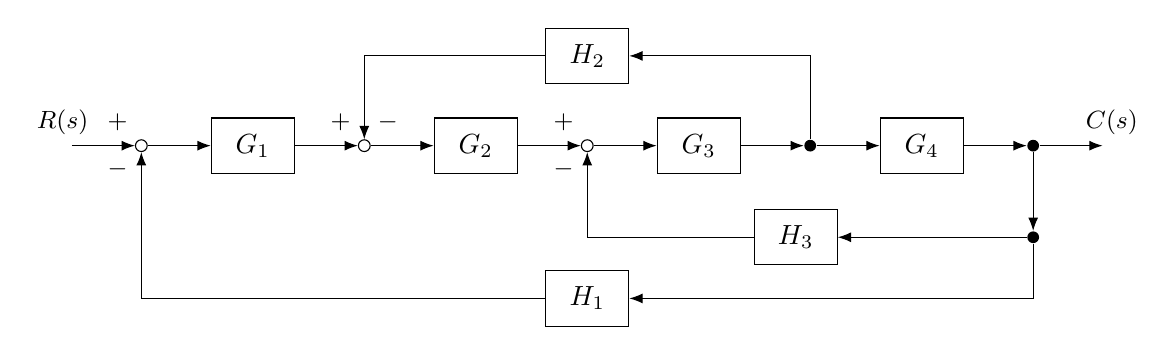
\begin{tikzpicture}[auto, node distance=0.8cm and 0.8cm, >=Latex]

    % --- 横並び:主系列ノード ---
    \node at (0,0) (input) {};
    \node[circle, draw, inner sep=1.5pt, right=of input] (sum1) {};         % 合流1
    \node[block, right=of sum1] (G1) {$G_1$};
    \node[circle, draw, inner sep=1.5pt, right=of G1] (sum2) {};            % 合流2
    \node[block, right=of sum2] (G2) {$G_2$};
    \node[circle, draw, inner sep=1.5pt, right=of G2] (sum3) {};            % 合流3
    \node[block, right=of sum3] (G3) {$G_3$};
    \node[circle, fill=black, inner sep=1.5pt, right=of G3] (branch1) {};   % 分岐1
    \node[block, right=of branch1] (G4) {$G_4$};
    \node[circle, fill=black, inner sep=1.5pt, right=of G4] (branch2) {};   % 分岐2
    \node[right=of branch2] (output) {};

    % --- 上・下ノード配置 ---
    \node[block, above=0.7cm of sum3] (H2) {$H_2$};                       % 合流3の上:H2
    \node[circle, fill=black, inner sep=1.5pt, below=1.0cm of branch2] (branch3) {}; % 分岐3
    \node[block, left=2.4cm of branch3] (H3) {$H_3$};                     % 分岐3の左
    \node[block, below=1.5cm of sum3] (H1) {$H_1$};                       % 合流3の下(H3より下)

    % === 主経路 ===
    \draw[->] (input) -- (sum1);
    \draw[->] (sum1) -- (G1);
    \draw[->] (G1) -- (sum2);
    \draw[->] (sum2) -- (G2);
    \draw[->] (G2) -- (sum3);
    \draw[->] (sum3) -- (G3);
    \draw[->] (G3) -- (branch1);
    \draw[->] (branch1) -- (G4);
    \draw[->] (G4) -- (branch2);
    \draw[->] (branch2) -- (output);

    % === 分岐ルート ===
    \draw[->] (branch1) |- (H2);              % 分岐1 → H2
    \draw[->] (H2) -| (sum2);                 % H2 → 合流2

    \draw[->] (branch2) -- (branch3);         % 分岐2 → 分岐3
    \draw[->] (branch3) -- (H3);              % 分岐3 → H3
    \draw[->] (H3) -| (sum3);                 % H3 → 合流3

    \draw[->] (branch3) |- (H1);              % 分岐3 → H1(下)
    \draw[->] (H1) -| (sum1);                 % H1 → 合流1

    % --- 加算記号配置 ---
    \node at ($(sum1)+(-0.3,0.3)$) {\small $+$};
    \node at ($(sum1)+(-0.3,-0.3)$) {\small $-$};

    \node at ($(sum2)+(-0.3,0.3)$) {\small $+$};
    \node at ($(sum2)+(+0.3,+0.3)$) {\small $-$};

    \node at ($(sum3)+(-0.3,0.3)$) {\small $+$};
    \node at ($(sum3)+(-0.3,-0.3)$) {\small $-$};

    % --- その他記号配置 ---
    \node at ($(sum1)+(-1.0,0.3)$) {\small $R(s)$};
    \node at ($(branch2)+(1.0,0.3)$) {\small $C(s)$};

\end{tikzpicture}
\end{center}
\vspace{2mm}


\noindent
[50] ブロック線図を簡単にせよ. 
\vspace{-2mm}
\begin{center}
    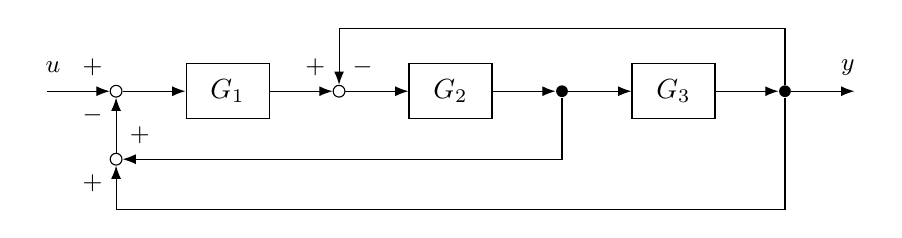
\begin{tikzpicture}[auto, node distance=0.8cm and 0.8cm, >=Latex]

    % --- 横並びの主系列ノード ---
    \node at (0,0) (input) {};
    \node[circle, draw, inner sep=1.5pt, right=of input] (sum1) {};         % 合流1
    \node[block, right=of sum1] (G1) {$G_1$};
    \node[circle, draw, inner sep=1.5pt, right=of G1] (sum2) {};            % 合流2
    \node[block, right=of sum2] (G2) {$G_2$};
    \node[circle, fill=black, inner sep=1.5pt, right=of G2] (branch1) {};   % 分岐1
    \node[block, right=of branch1] (G3) {$G_3$};
    \node[circle, fill=black, inner sep=1.5pt, right=of G3] (branch2) {};   % 分岐2
    \node[right=of branch2] (output) {};
    
    % --- 合流3(sum1の下) ---
    \node[circle, draw, inner sep=1.5pt, below=0.7cm of sum1] (sum3) {};    % 合流3
    
    % === 経路 ===
    \draw[->] (input) -- (sum1);
    \draw[->] (sum1) -- (G1);
    \draw[->] (G1) -- (sum2);
    \draw[->] (sum2) -- (G2);
    \draw[->] (G2) -- (branch1);
    \draw[->] (branch1) -- (G3);
    \draw[->] (G3) -- (branch2);
    \draw[->] (branch2) -- (output);
    
    \draw[->] (branch1) |- (sum3);      % 分岐1 → 合流3
    \draw[->] (sum3) -- (sum1);         % 合流3 → 合流1
    
    \draw[->] (branch2) |- ++(0,-1.5) -| (sum3);   % 分岐2 → 合流3(下経路)
    \draw[->] (branch2) |- ++(0,0.8) -| (sum2);    % 分岐2 → 合流2(上経路)
    
    % --- 加算記号配置 ---
    \node at ($(sum1)+(-0.3,0.3)$) {\small $+$};
    \node at ($(sum1)+(-0.3,-0.3)$) {\small $-$};
    \node at ($(sum2)+(-0.3,0.3)$) {\small $+$};
    \node at ($(sum2)+(0.3,0.3)$) {\small $-$};
    \node at ($(sum3)+(0.3,0.3)$) {\small $+$};
    \node at ($(sum3)+(-0.3,-0.3)$) {\small $+$};
    
    % --- その他記号配置 ---
    \node at ($(sum1)+(-0.8,0.3)$) {\small $u$};
    \node at ($(branch2)+(0.8,0.3)$) {\small $y$};
    
\end{tikzpicture}
\end{center}
\vspace{1mm}


\end{document}
